\documentclass[english,a4,aspectratio=169]{beamer}
\usepackage[T1]{fontenc}
\usepackage[utf8]{inputenc}
\setcounter{secnumdepth}{3}
\setcounter{tocdepth}{3}
\usepackage{array}
\usepackage{graphicx}
\usepackage{tabularx}
\usepackage{pgfpages}
\usepackage{bm}
\usepackage{eurosym}
\usepackage{amsmath}
\usepackage{cancel}
\usepackage{color}
\usepackage{comment}

\setbeamertemplate{footline}[frame number]

\newcommand{\argmax}{\mathop{\mathrm{arg\,max}}}
\newcommand{\argmin}{\mathop{\mathrm{arg\,min}}}

\usepackage{tikz}
\usetikzlibrary{arrows}
%\pgfpagesuselayout{resize to}[a4paper,landscape]

%thse two commands are important for Calvin's slides
%\usepackage{tikz}
%\usetikzlibrary{arrows,decorations.pathmorphing,backgrounds,positioning,fit,petri,intersections}


% %%%%%%%%%%%%%%%%%%%%%%%%%%%%%% User specified LaTeX commands.
%\usepackage[size=a4]{beamerposter}

% points to drive home:
%
% Markov model talk was trying to drive home the relationship to probability theory and linear algebra
% Here we'll talk about the relationship to Bayesian statistics

\title{How Zalando Accelerates Warehouse Operations with Neural Networks}
\author{Calvin Seward\\Big Data Berlin v.\ 6.0}
\date{28 January 2016}
\institute{
\includegraphics[width=6cm]{../figures/logo_zalando_all_sRGB.jpg}}

\usepackage{babel}
\begin{document}


\begin{frame}
 \maketitle
\end{frame}
\logo{
\includegraphics[width=2cm]{../figures/zalandoLogo.jpg}\quad}

\begin{frame}
 \frametitle{Outline}
 \begin{itemize}
  \item Picker Routing Problem
  \item Order Batching Problem
  \item Neural Network Estimate of Pick Route Length
  \item Order Batch optimization via Simulated Annealing
 \end{itemize}
\onslide<2->
\quad\\
This was a project that was a collaboration between Rolland Vollgraf, Sebastian Heinz and myself.  Some of the figures have been shamelessly stolen from Roland.
\end{frame}

\begin{frame}
\frametitle{Zalando's Logistics Centers}
 \begin{itemize}
  \item 13.8 Million orders from 01.07.15 -- 30.09.15
  \item 174,684 orders send per working day (Mo.\ -- Sa.)
  \item Every second handling time per order requires 160 man-days of work / month
  \item Any increase in efficency has a big impact
 \end{itemize}
\end{frame}

\begin{comment}
\begin{frame}
\frametitle{Picker Routing Problem}
\framesubtitle{The Pick Route}
 \begin{figure}
  \centering
  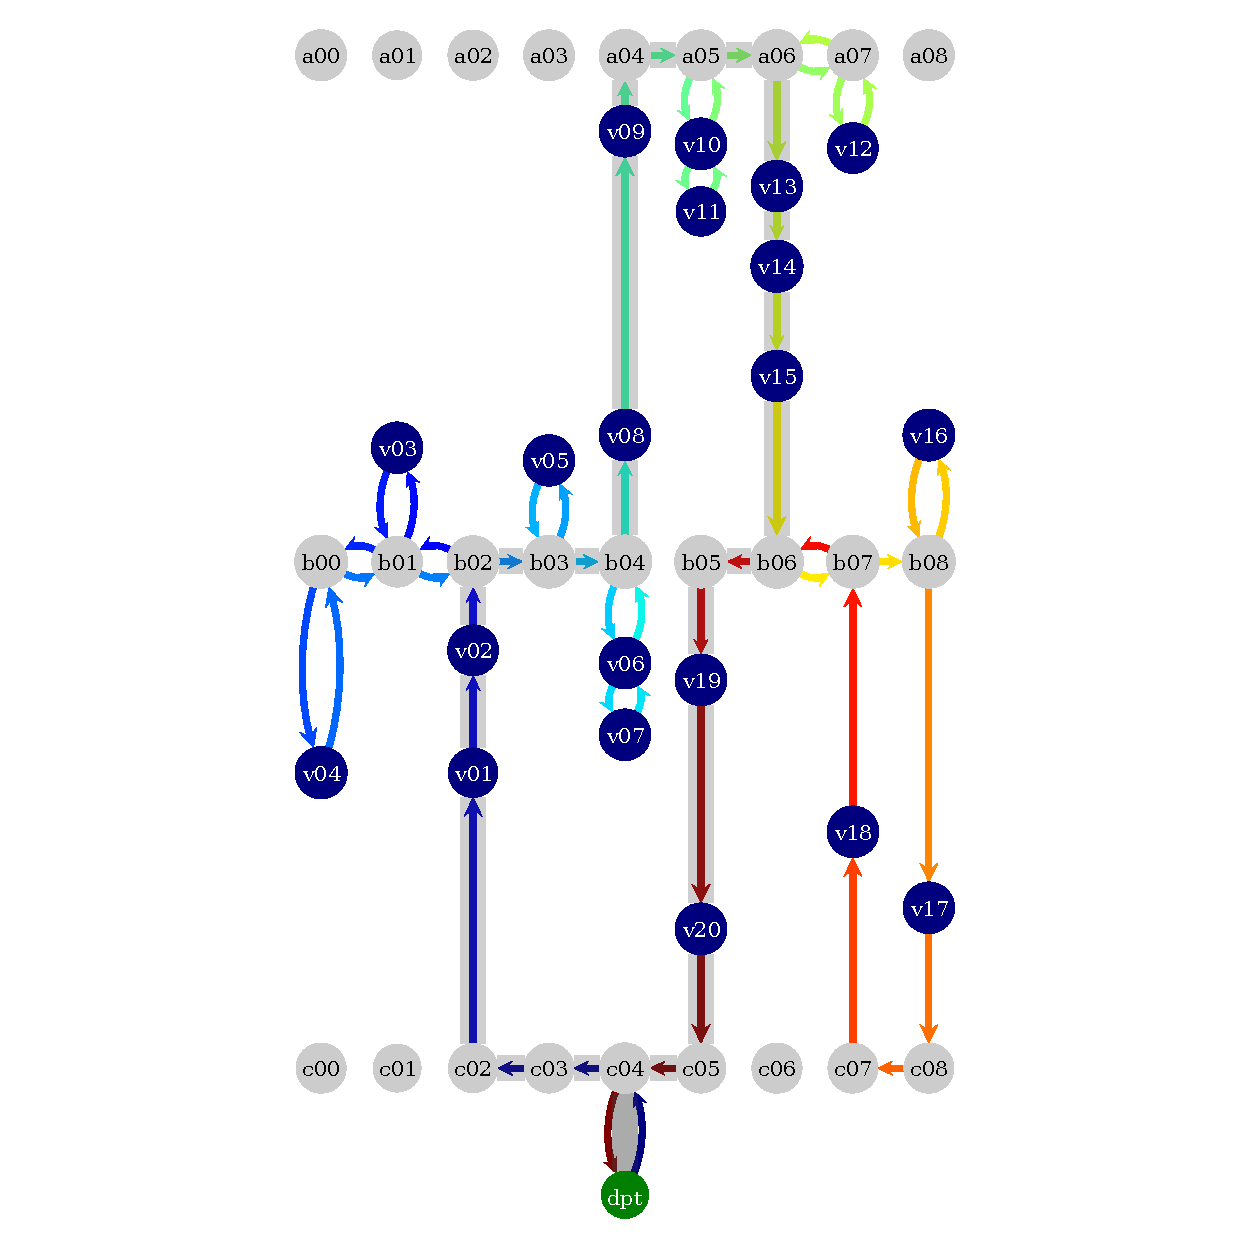
\includegraphics[height=.6\textheight]{figures/loop_example.pdf}
 \end{figure}
\end{frame}
\end{comment}

\begin{frame}
\frametitle{Picker Routing Problem}
\framesubtitle{The locations that must be visited}
 \begin{figure}
  \centering
  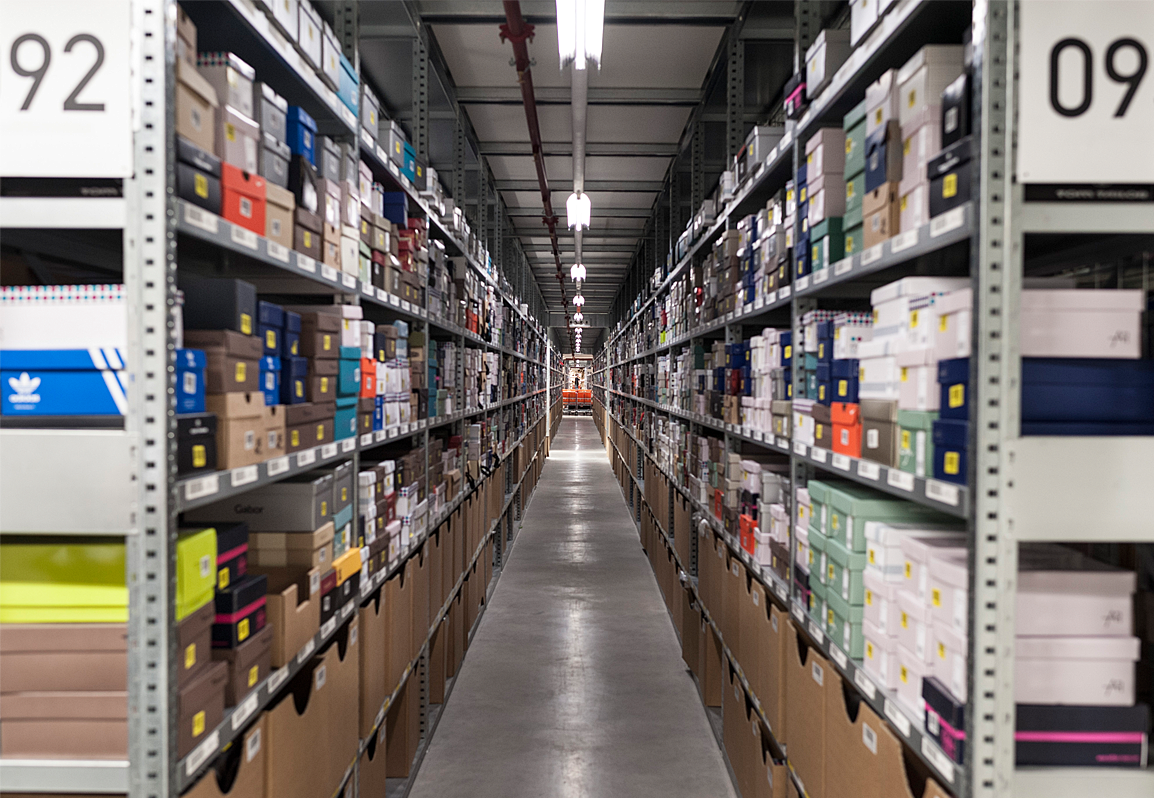
\includegraphics[width=.65\textwidth]{../figures/retail_3_gross.png}
 \end{figure}
\end{frame}

\begin{frame}
\frametitle{Picker Routing Problem}
\framesubtitle{The locations that must be visited}
 \begin{figure}
  \centering
  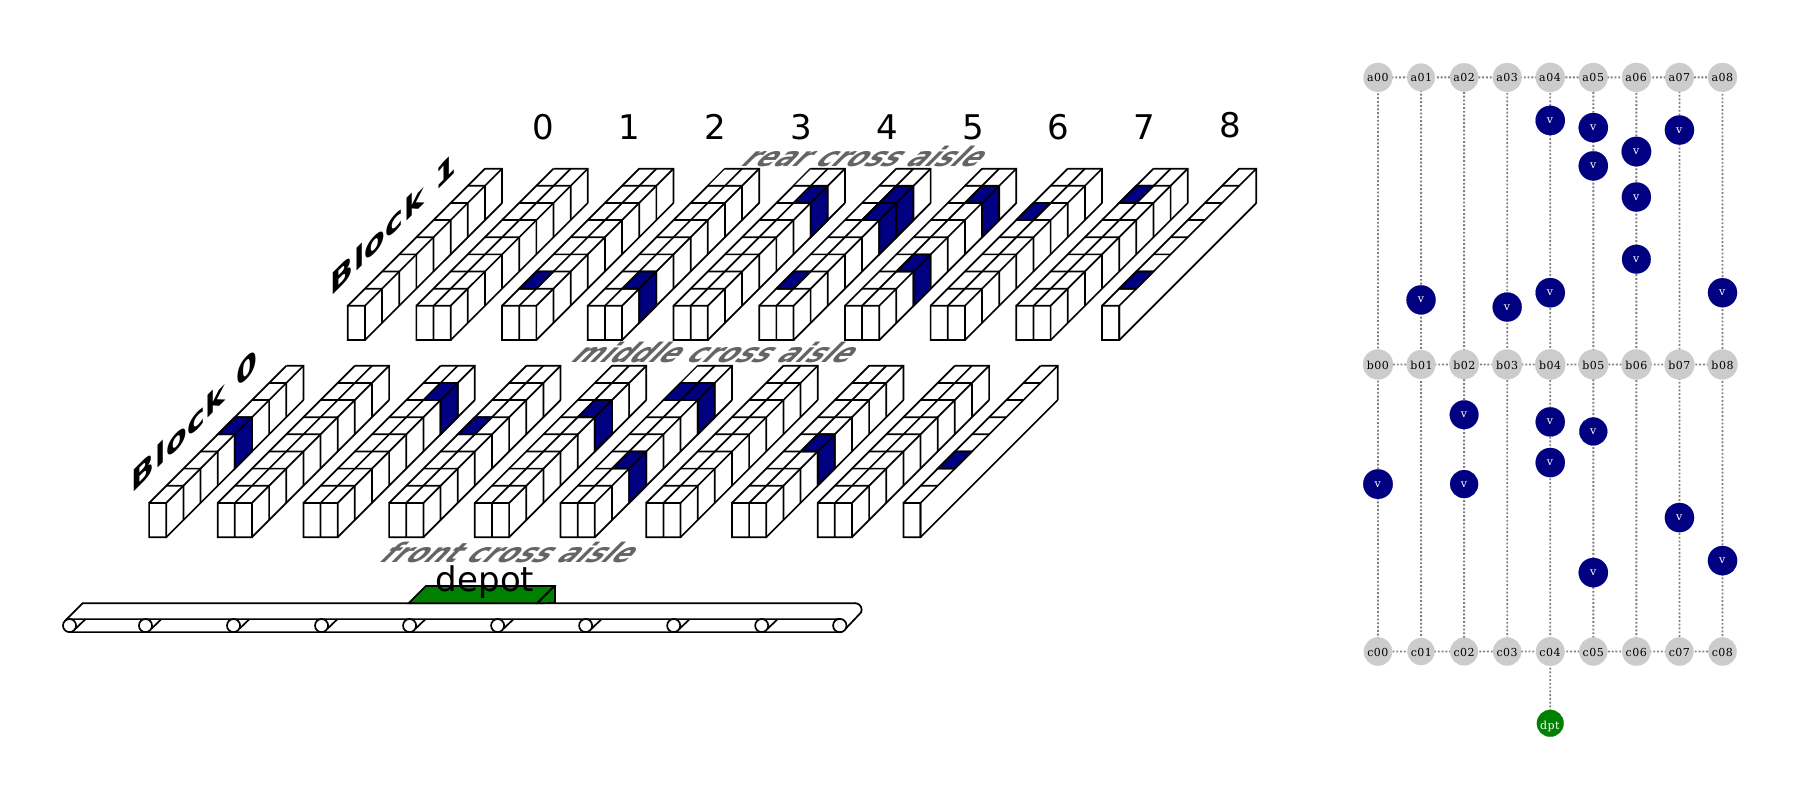
\includegraphics[width=\textwidth]{../figures/warehouse_3d.png}
 \end{figure}
\end{frame}

\begin{frame}
\frametitle{Picker Routing Problem}
\framesubtitle{The Pick Route}
 \begin{figure}
  \centering
  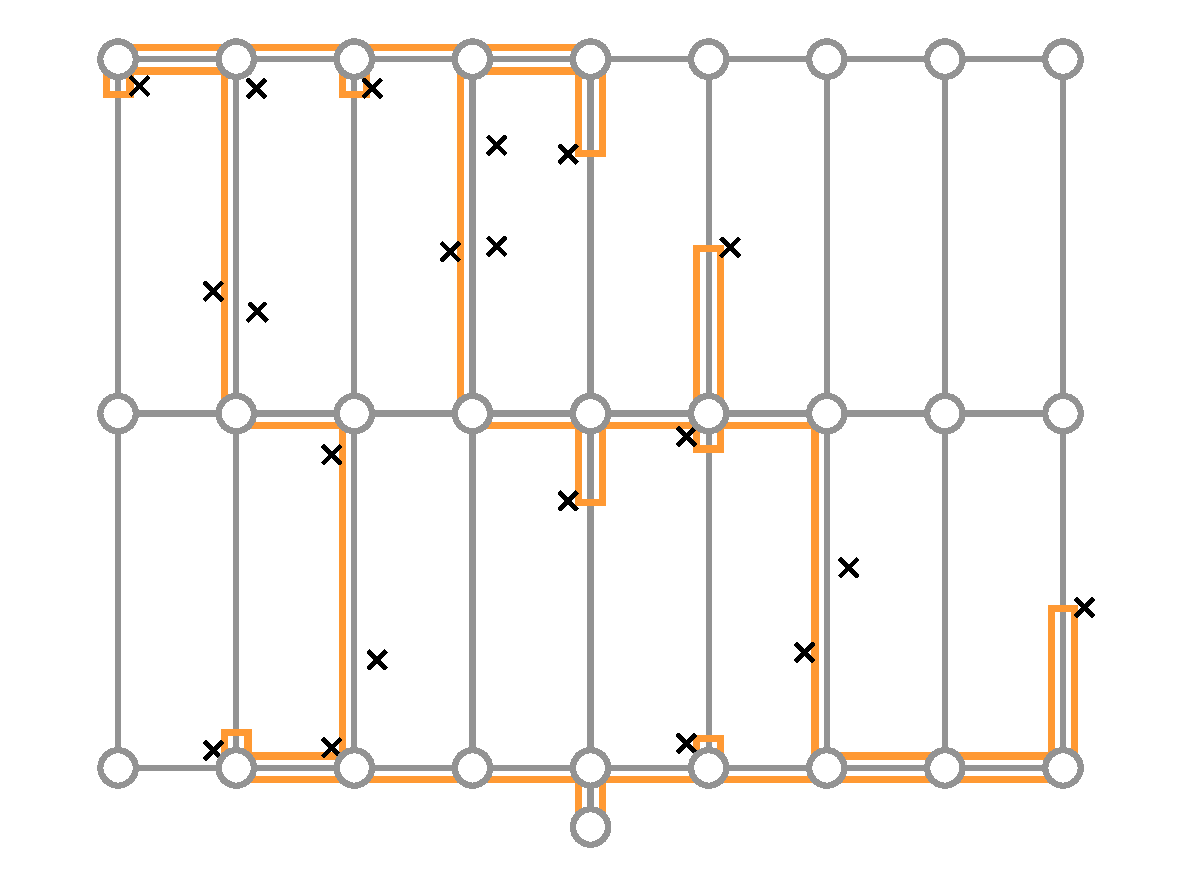
\includegraphics[width=.6\textwidth]{../figures/route_optimal.pdf}
 \end{figure}
\end{frame}

\begin{frame}
\frametitle{Picker Routing Problem}
\framesubtitle{The Pick Route}
 \begin{figure}
  \centering
  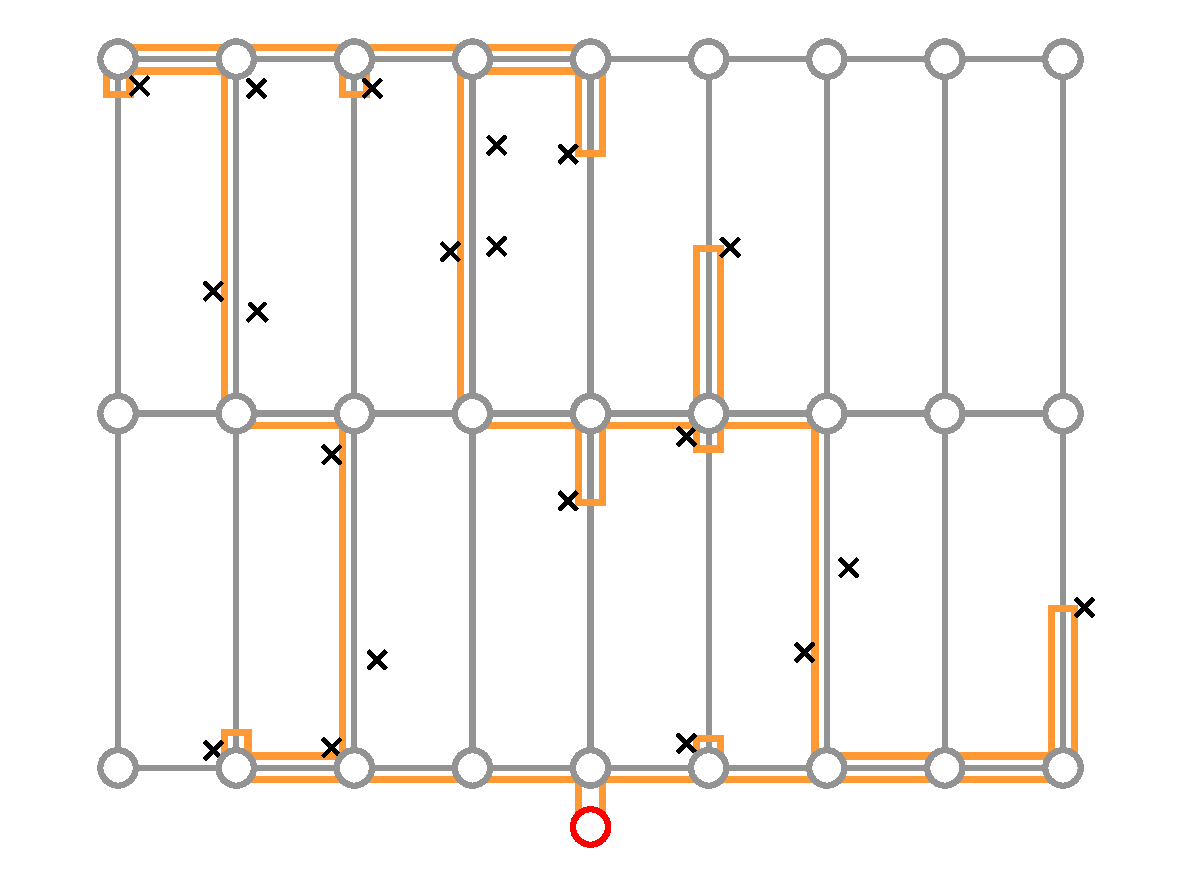
\includegraphics[width=.6\textwidth]{../figures/path01.pdf}
 \end{figure}
\end{frame}

\begin{frame}
\frametitle{Picker Routing Problem}
\framesubtitle{The Pick Route}
 \begin{figure}
  \centering
  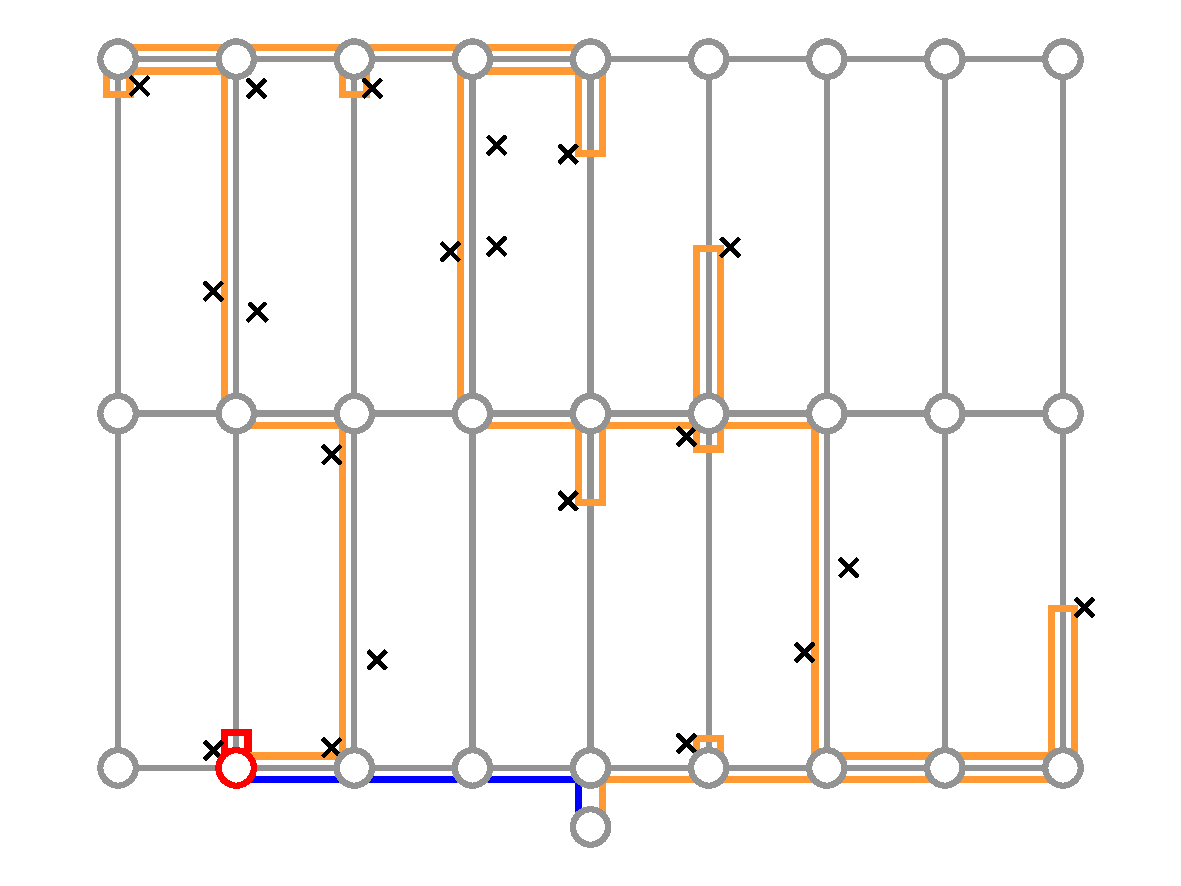
\includegraphics[width=.6\textwidth]{../figures/path07.pdf}
 \end{figure}
\end{frame}

\begin{frame}
\frametitle{Picker Routing Problem}
\framesubtitle{The Pick Route}
 \begin{figure}
  \centering
  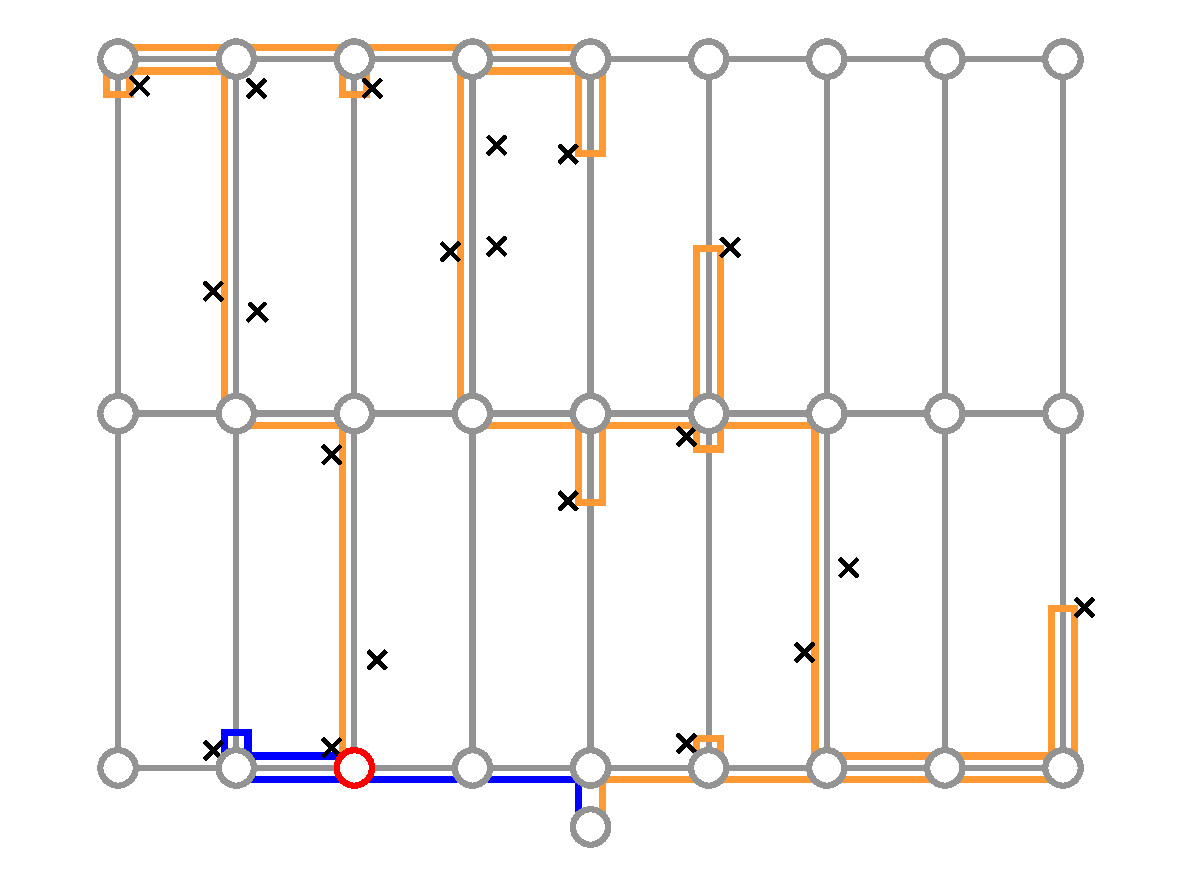
\includegraphics[width=.6\textwidth]{../figures/path09.pdf}
 \end{figure}
\end{frame}

\begin{frame}
\frametitle{Picker Routing Problem}
\framesubtitle{The Pick Route}
 \begin{figure}
  \centering
  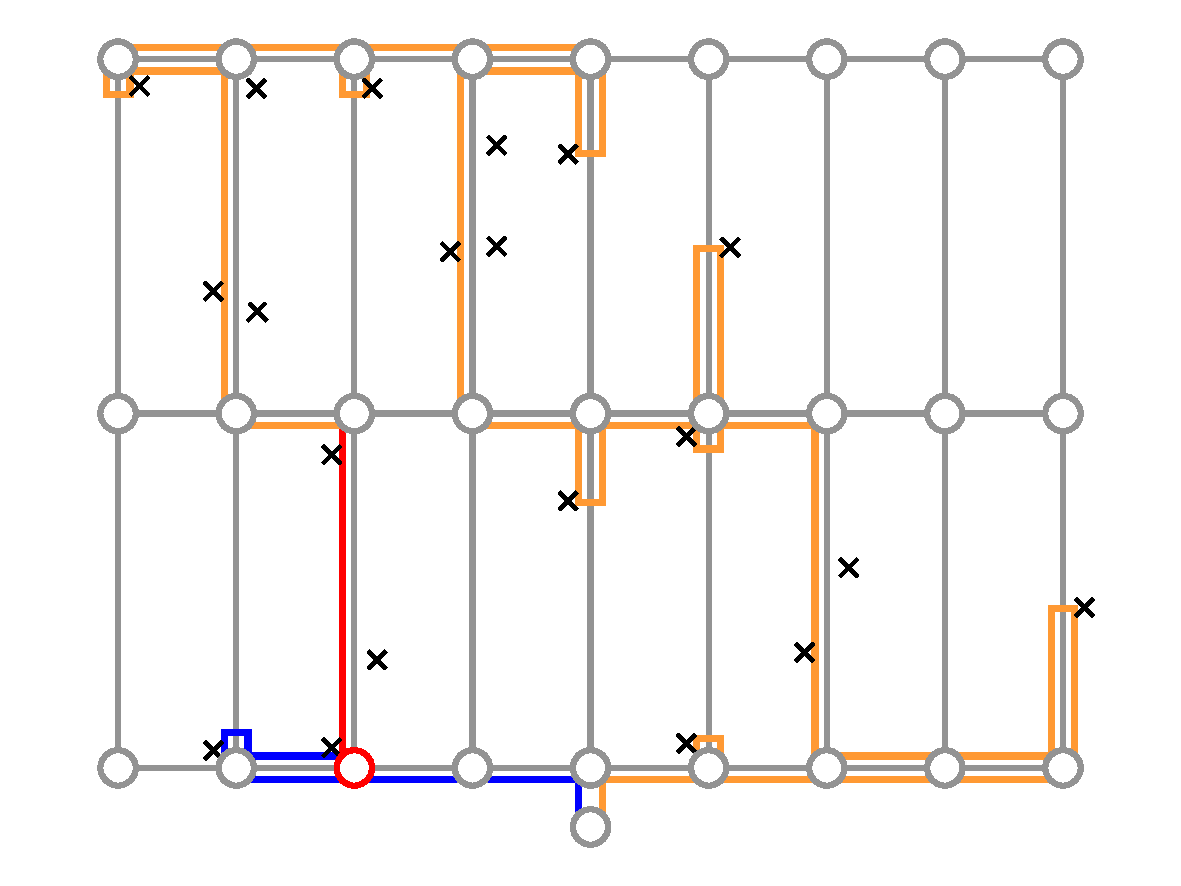
\includegraphics[width=.6\textwidth]{../figures/path10.pdf}
 \end{figure}
\end{frame}

\begin{frame}
\frametitle{Picker Routing Problem}
\framesubtitle{The Pick Route}
 \begin{figure}
  \centering
  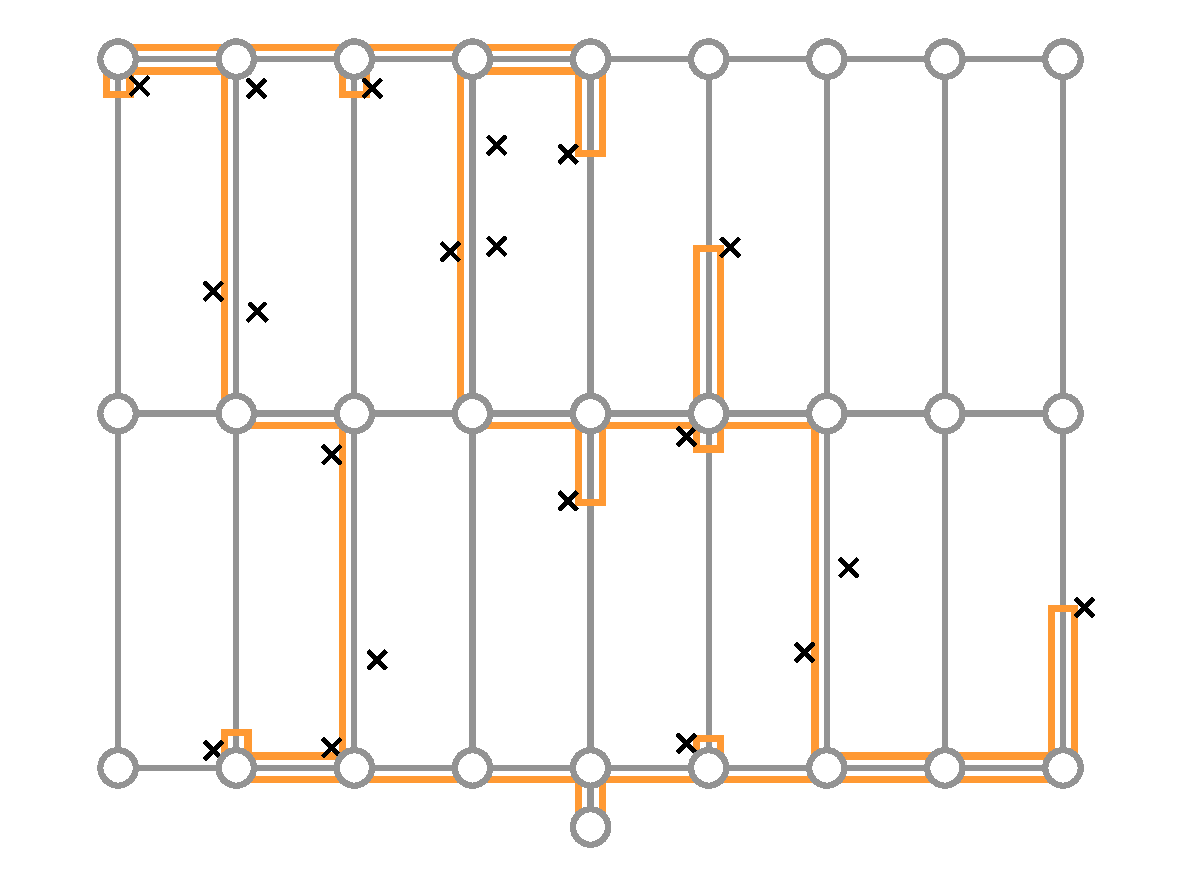
\includegraphics[width=.6\textwidth]{../figures/route_optimal.pdf}
 \end{figure}
\end{frame}

\begin{frame}
\frametitle{OCaPi Algorithm}
\framesubtitle{Optimal CArt PIck}
\begin{columns}[c]
\column{.5\textwidth}
\begin{itemize}
 \item To solve picker routing problem, we developed the OCaPi Algorithm
 \item Calculates the optimal route to walk
 \item Also determines optimal cart handling strategy
 \item<2-> Has complexity that is linear in the number of aisles
 \item<3-> Unfortunately still has a runtime of around 1 second
\end{itemize}
\column{.5\textwidth}
 \begin{figure}
  \centering
  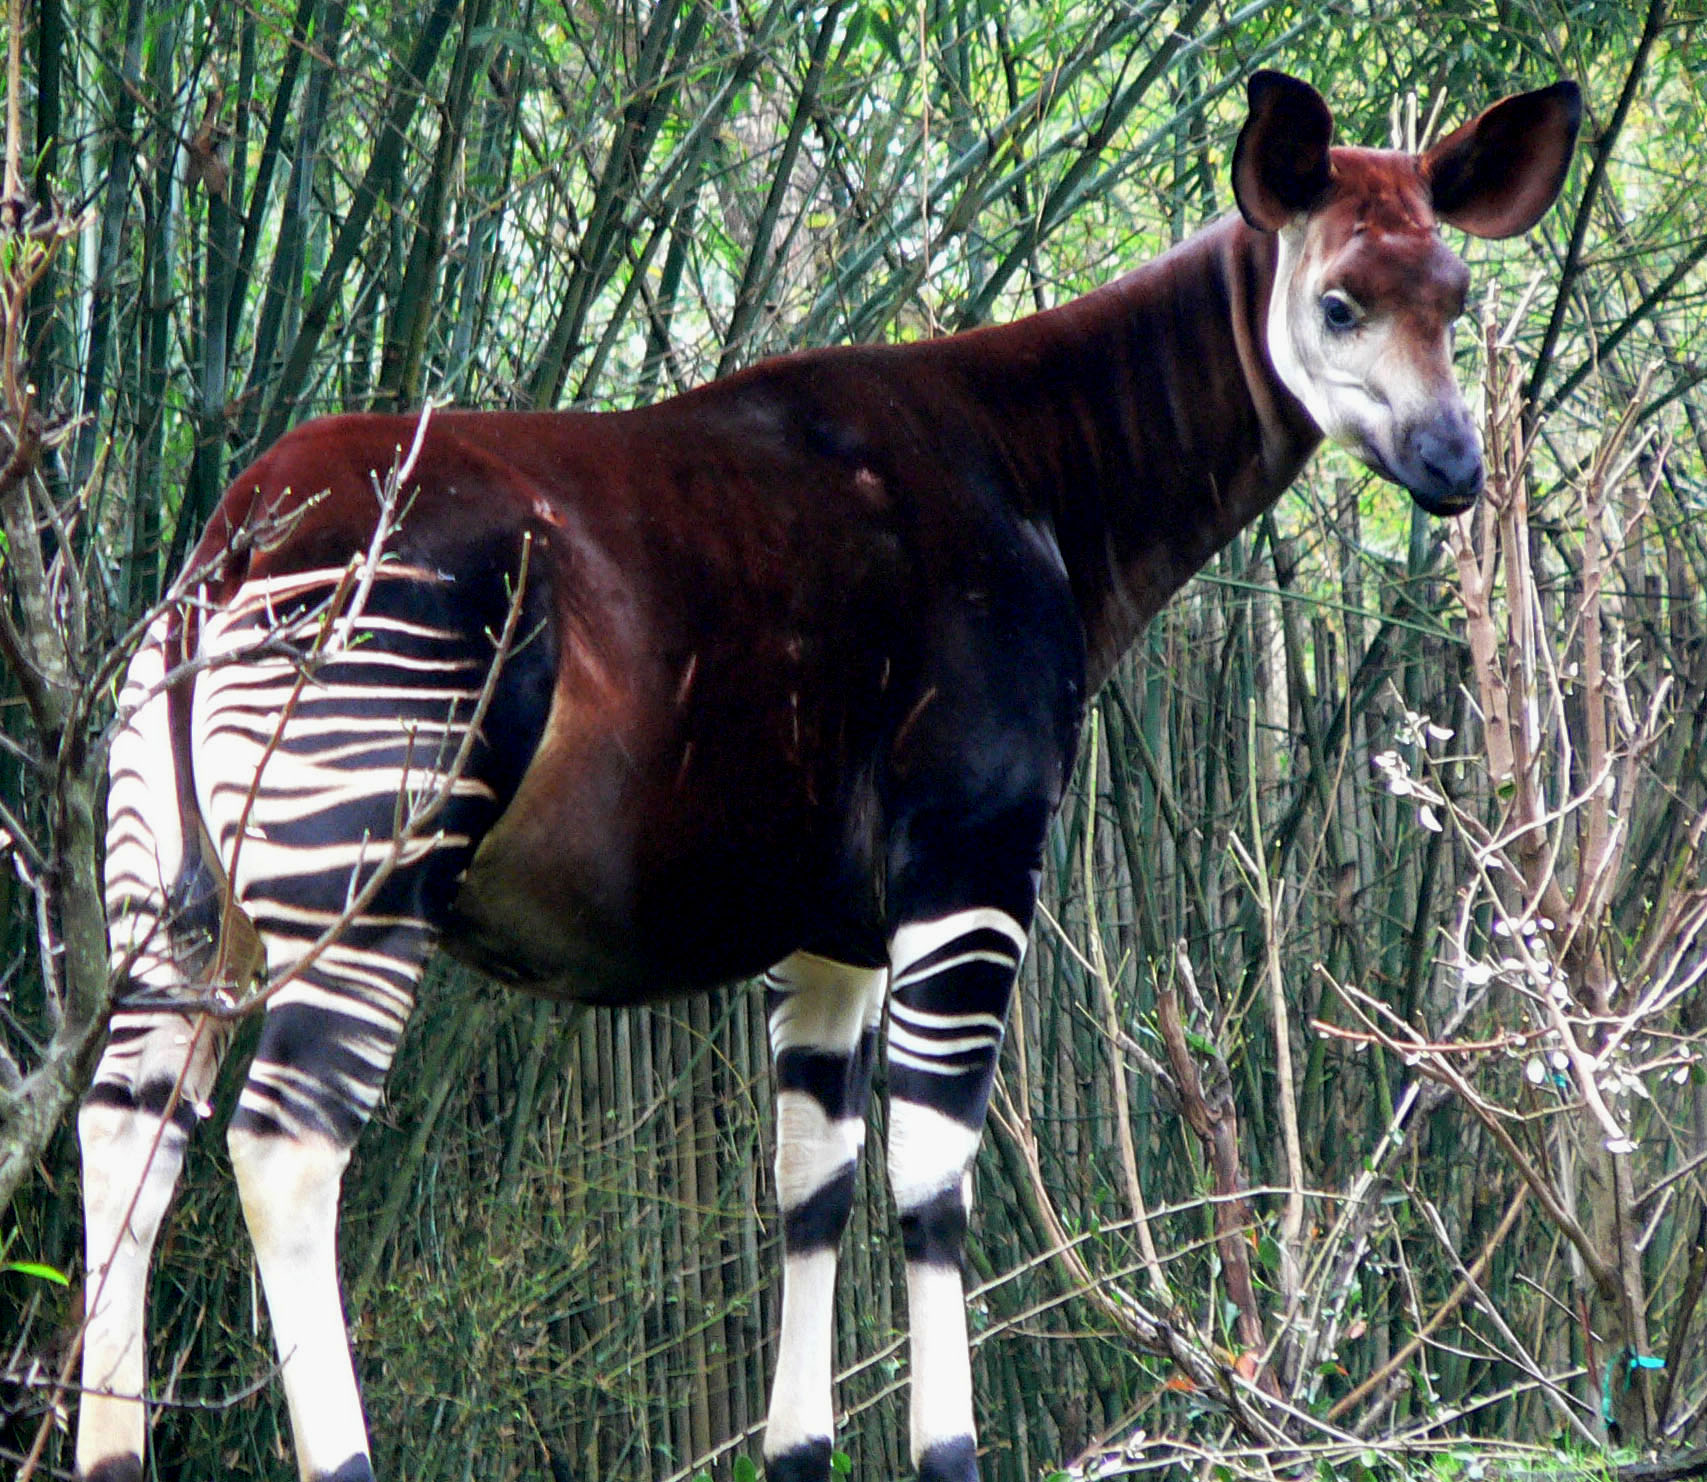
\includegraphics[width=.7\textwidth]{../figures/Okapi2.jpg}
  \caption{The Okapi -- Our Mascot}
 \end{figure}
 \end{columns}
\end{frame}

\begin{frame}
 \frametitle{Simplified Order Batching Problem}
 \framesubtitle{Bipartite Graph Formulation}
 
 \begin{figure}
 \centering
 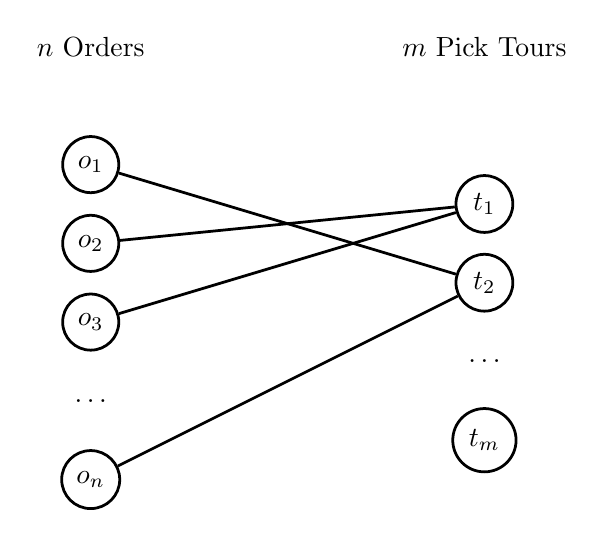
\begin{tikzpicture}[scale=.25,draw,line width=1pt]
  \path (0cm,6cm)         node (x) {$n$ Orders};
  \path (0cm,0cm)          node[draw,shape=circle] (o1) {$o_1$};
  \path (0cm,-4cm)          node[draw,shape=circle] (o2) {$o_2$};
  \path (0cm,-8cm)          node[draw,shape=circle] (o3) {$o_3$};
  \path (0cm,-12cm)          node[shape=circle] (x2) {$\hdots$};
  \path (0cm,-16cm)          node[draw,shape=circle] (on) {$o_n$};
  \path (20cm,6cm)        node (y) {$m$ Pick Tours};
  \path (20cm,-2cm)         node[draw,shape=circle] (t1) {$t_1$};
  \path (20cm,-6cm)         node[draw,shape=circle] (t2) {$t_2$};
  \path (20cm,-10cm)          node[shape=circle] (y2) {$\hdots$};
  \path (20cm,-14cm)         node[draw,shape=circle] (t3) {$t_m$};
  \onslide<2->
  \draw[line width=1pt] (o1) -- (t2);
  \onslide<3->
  \draw[line width=1pt] (o3) -- (t1);
  \onslide<3->
  \draw[line width=1pt] (o2) -- (t1);
  \draw[line width=1pt] (on) -- (t2);
 \end{tikzpicture}
 \end{figure}
\end{frame}

\begin{frame}
\frametitle{Order Batching Problem}
\framesubtitle{Random Split of 10 Orders \`a 2 Items Into Two Pick Routes}
 \begin{figure}
  \centering
  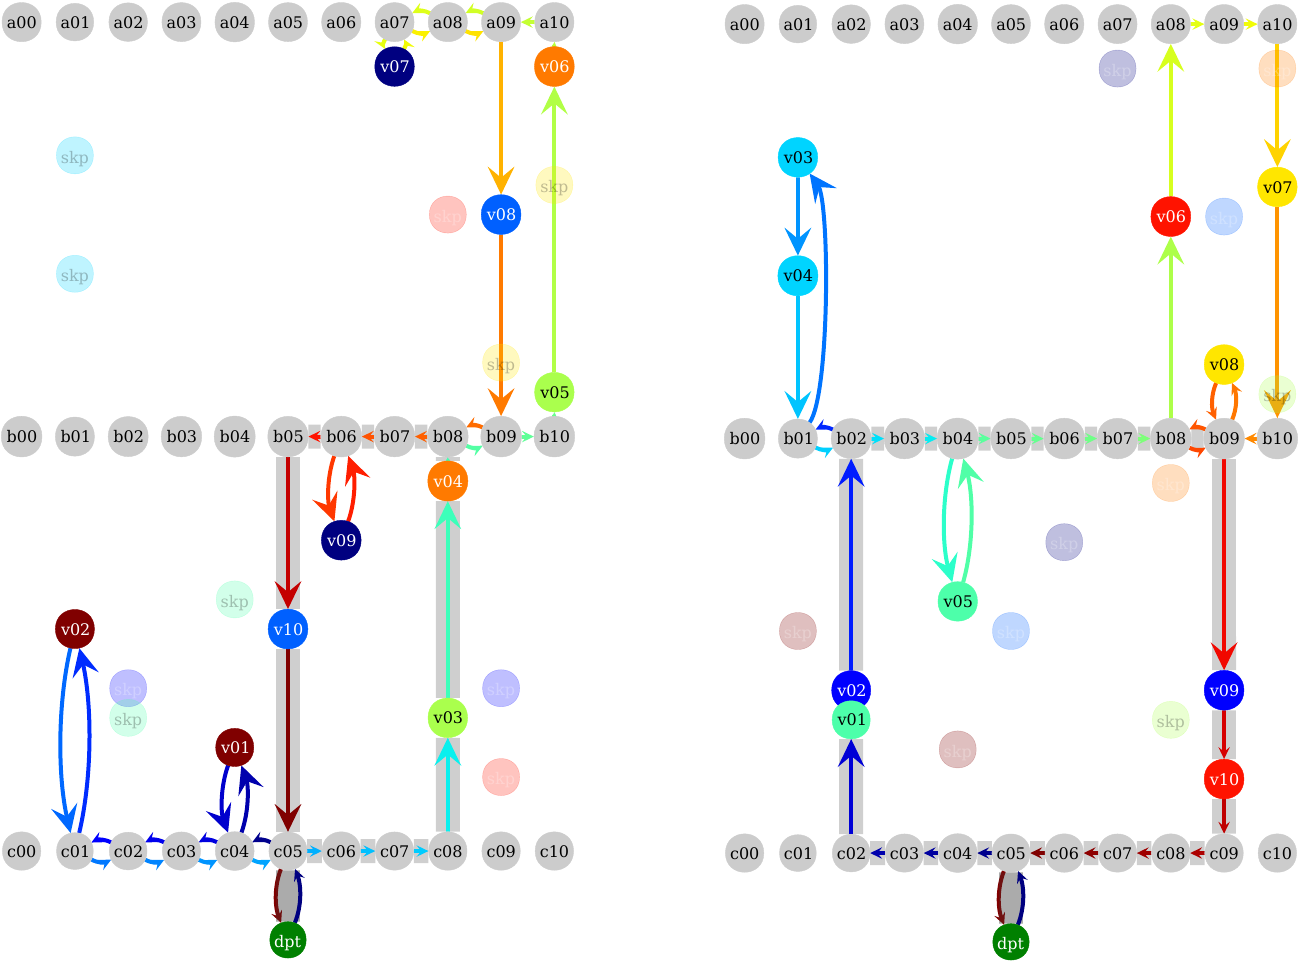
\includegraphics[width=.7\textwidth]{../figures/median.png}
 \end{figure}
\end{frame}

\begin{frame}
\frametitle{Order Batching Problem}
\framesubtitle{Brute Force Split of 10 Orders \`a 2 Items into Optimal Two Pick Routes $\rightarrow\;8.3\%$ Boost}
 \begin{figure}
  \centering
  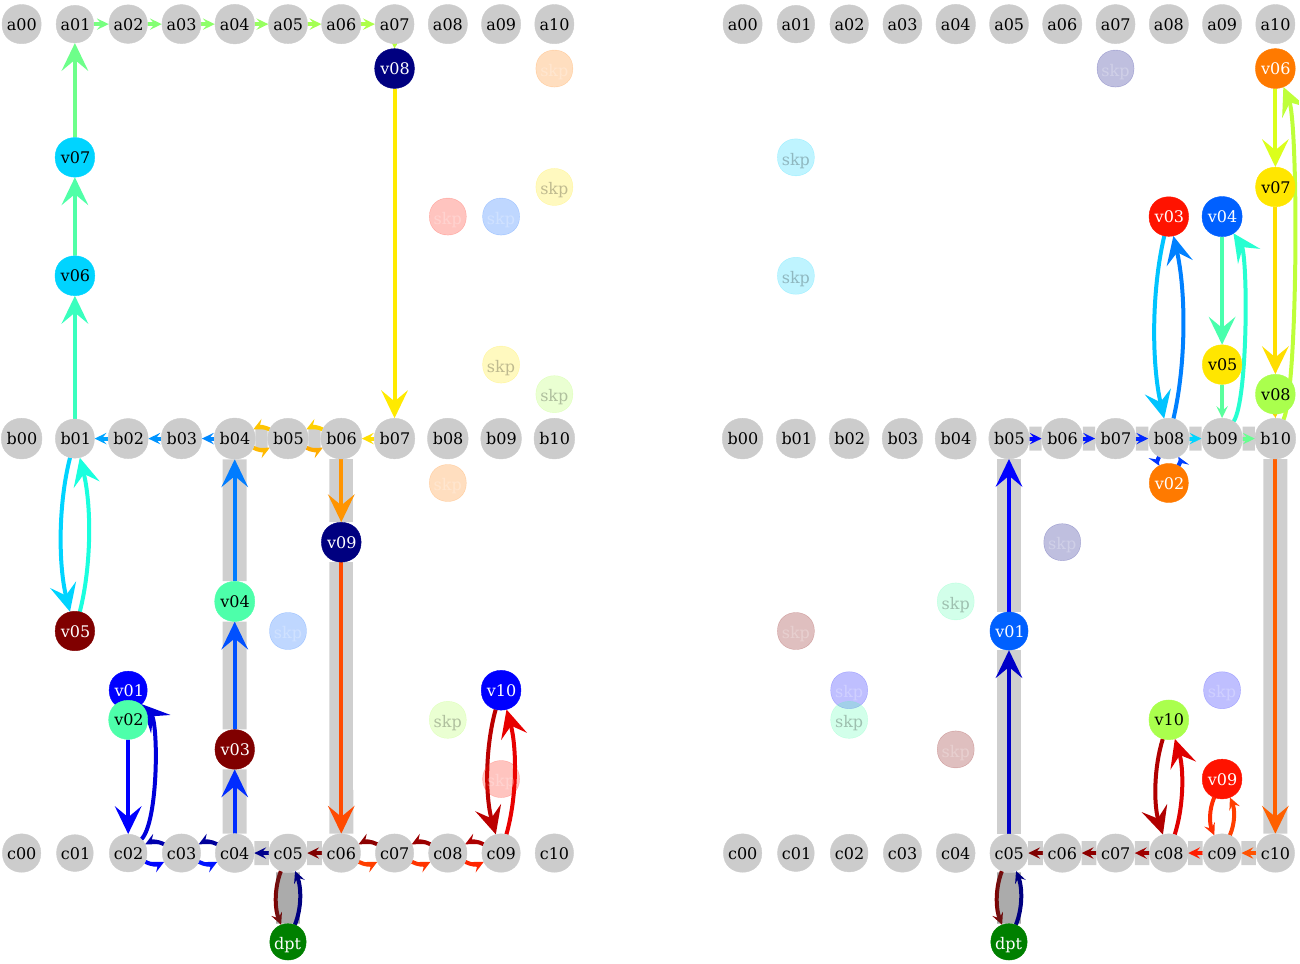
\includegraphics[width=.7\textwidth]{../figures/best.png}
 \end{figure}
\end{frame}

\begin{frame}
 \frametitle{Neural Network Estimate of Pick Route Length}
  \begin{columns}[c]
  \column{.5\textwidth}
  \begin{itemize}
   \item This simple example could be done with brute force
   \item A realistic example with 40 orders \`a 2 items has a complexity of
   \[\frac{40!}{2\cdot 20!\cdot 20!}\approx6.9\cdot 10^{10}\]
   at 1 second per route, you'd wait 2185 years
   \item<2-> Use clever heuristics like simulated annealing
   \item<2-> Estimate pick route length with Neural Networks 
  \end{itemize}
  \column{.5\textwidth}
  \end{columns}
\end{frame}

\begin{frame}
 \frametitle{Neural Network Estimate of Pick Route Length}
  \begin{columns}[c]
  \column{.6\textwidth}
  \begin{itemize}
  \item OCaPi cost landscape \[f:(\mathbb N\times\mathbb R)^n\to\mathbb R_+\] is a nice function because it is:
  \begin{itemize}
   \item Lipschitz continuous in the real-valued arguments
   \item Piecewise linear in the real-valued arguments
   \item Locally sensitive
  \end{itemize}
  \item<2-> Perfect function to model with Convolutional Neural Networks with ReLUs:
  \[\tilde f(x):=(W_2(W_1x+b_1)_{+} + b_2)_{+}\]
  \item<2-> Train convolutional neural network with 1 million examples
  \end{itemize}
  \column{.4\textwidth}
  \begin{figure}
   \centering
   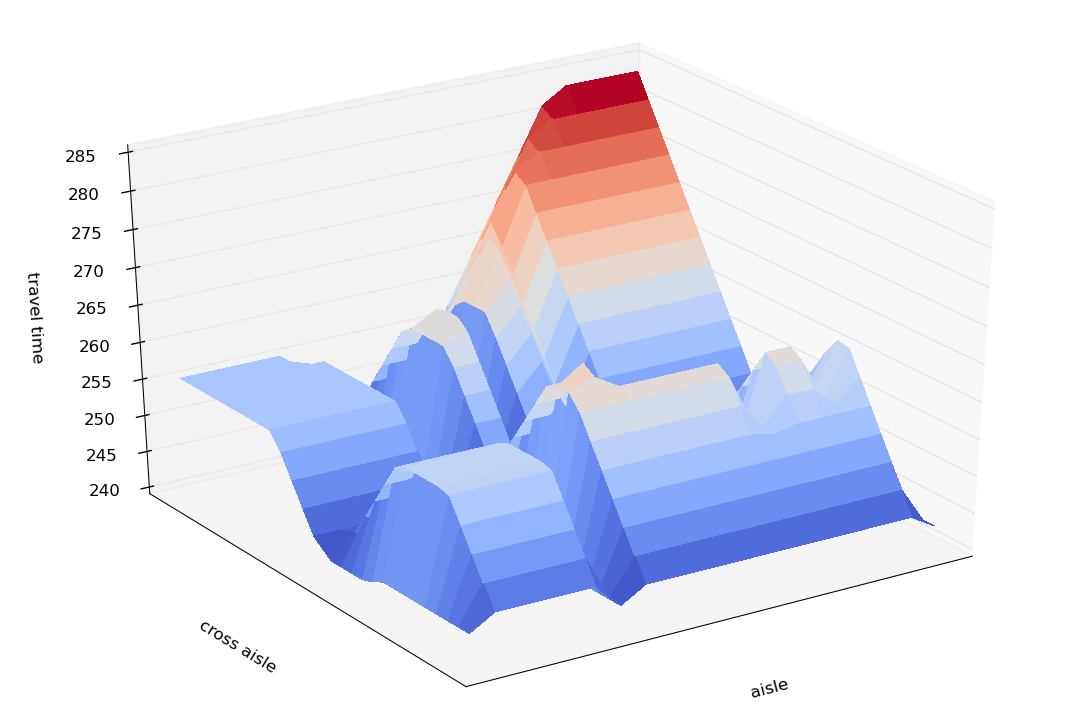
\includegraphics[width=\textwidth]{../figures/landscape_by_calvin.png}
   \end{figure}
  \end{columns}
\end{frame}

\begin{frame}
 \frametitle{Neural Network Estimate of Pick Route Length}
 \framesubtitle{Estimation Accuracy -- Frequency of relative estimation error $\;\;\frac{\text{estimated travel time}}{\text{calculated travel time}}$}
 \begin{figure}
  \centering
  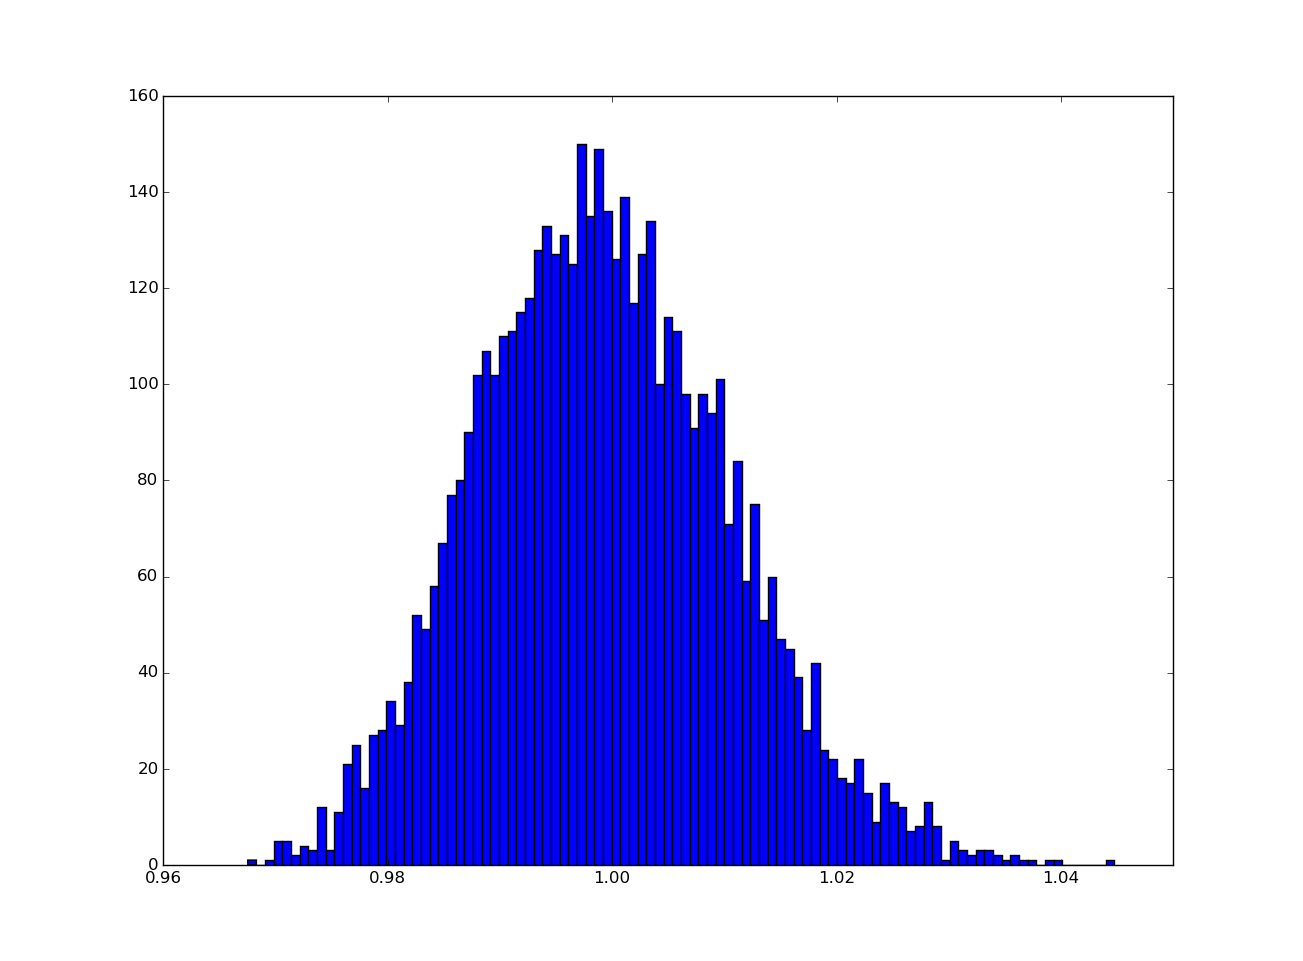
\includegraphics[height=.85\textheight]{../figures/estimation_error.png}
 \end{figure}
\end{frame}

\begin{frame}
 \frametitle{Neural Network Estimate of Pick Route Length}
 \framesubtitle{Estimation Speed -- Time Per Route on two Intel Xeon E5-2640 and two NVIDIA Tesla K80 accelerators}
 \begin{table}
  \begin{tabular}{l|lll}
number pick lists & OCaPi & CPU network & GPU network \\\hline
1    & 5.369 & 2.202e-3 & 1.656e-3 \\
10    & 1.326 & 1.991e-4 & 1.832e-4 \\
100   & 0.365 & 6.548e-5 & 5.919e-5 \\
1000  &       & 3.086e-5 & 2.961e-5 \\
10000 &       & 2.554e-5 & 2.336e-5
  \end{tabular}
 \end{table}
\end{frame}

\begin{frame}
 \frametitle{Order Batch optimization via Simulated Annealing}
 \framesubtitle{Estimated and Exact Improvement in Example Simulated Annealing Run}
 \begin{figure}
  \centering
  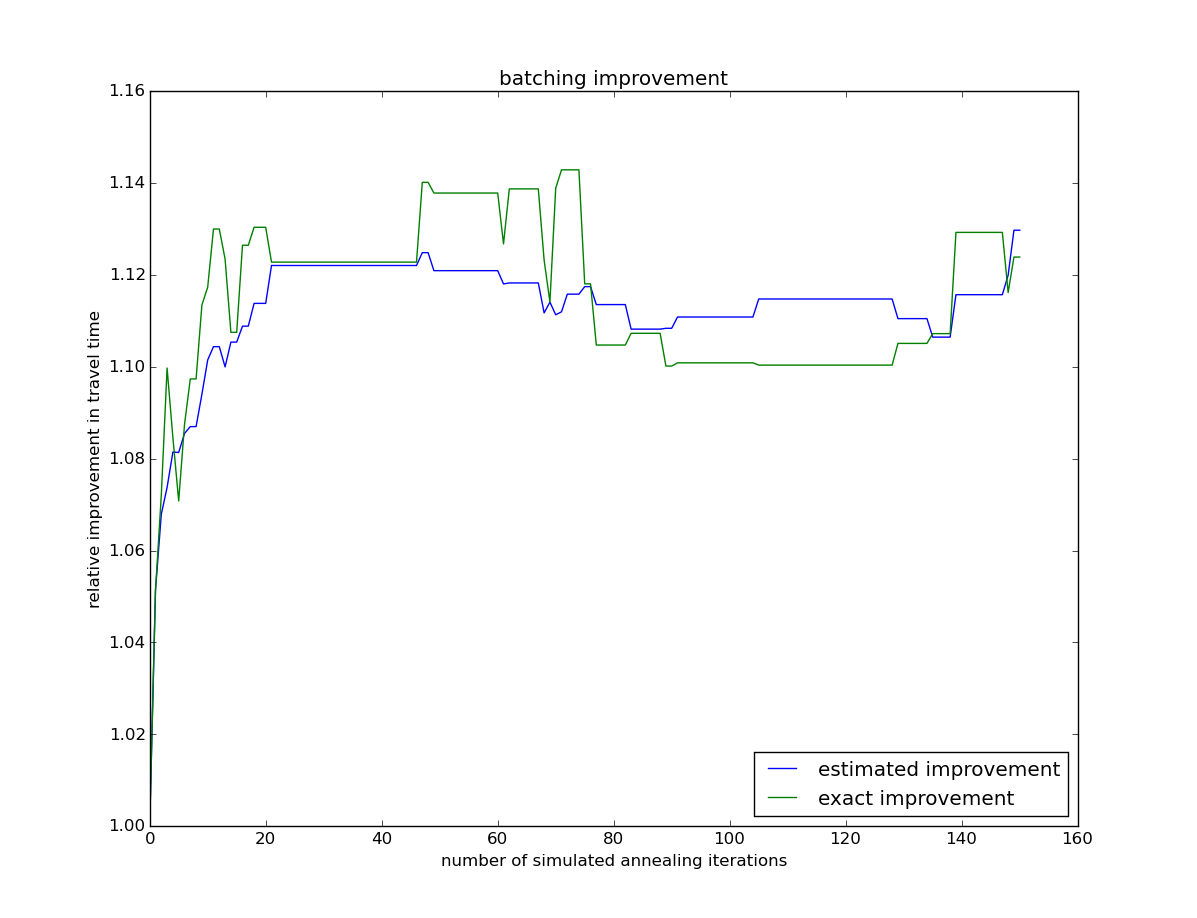
\includegraphics[height=.85\textheight]{../figures/sim_an_run.png}
 \end{figure}
\end{frame}

\begin{frame}
\begin{center}
 Questions?
\end{center}
\end{frame}

\logo{}
%%%%%%%%%%%%%%%%%%%%%%%%%%%%%%%%%%%%%%%%%%%%%%%%%%%%%%%%%%%%%%%%%%%%%%%%%%%%%%%%%%%%%%%%%%%%%%%%%%%%
\setbeamertemplate{background canvas}{
    \hspace{-.5cm}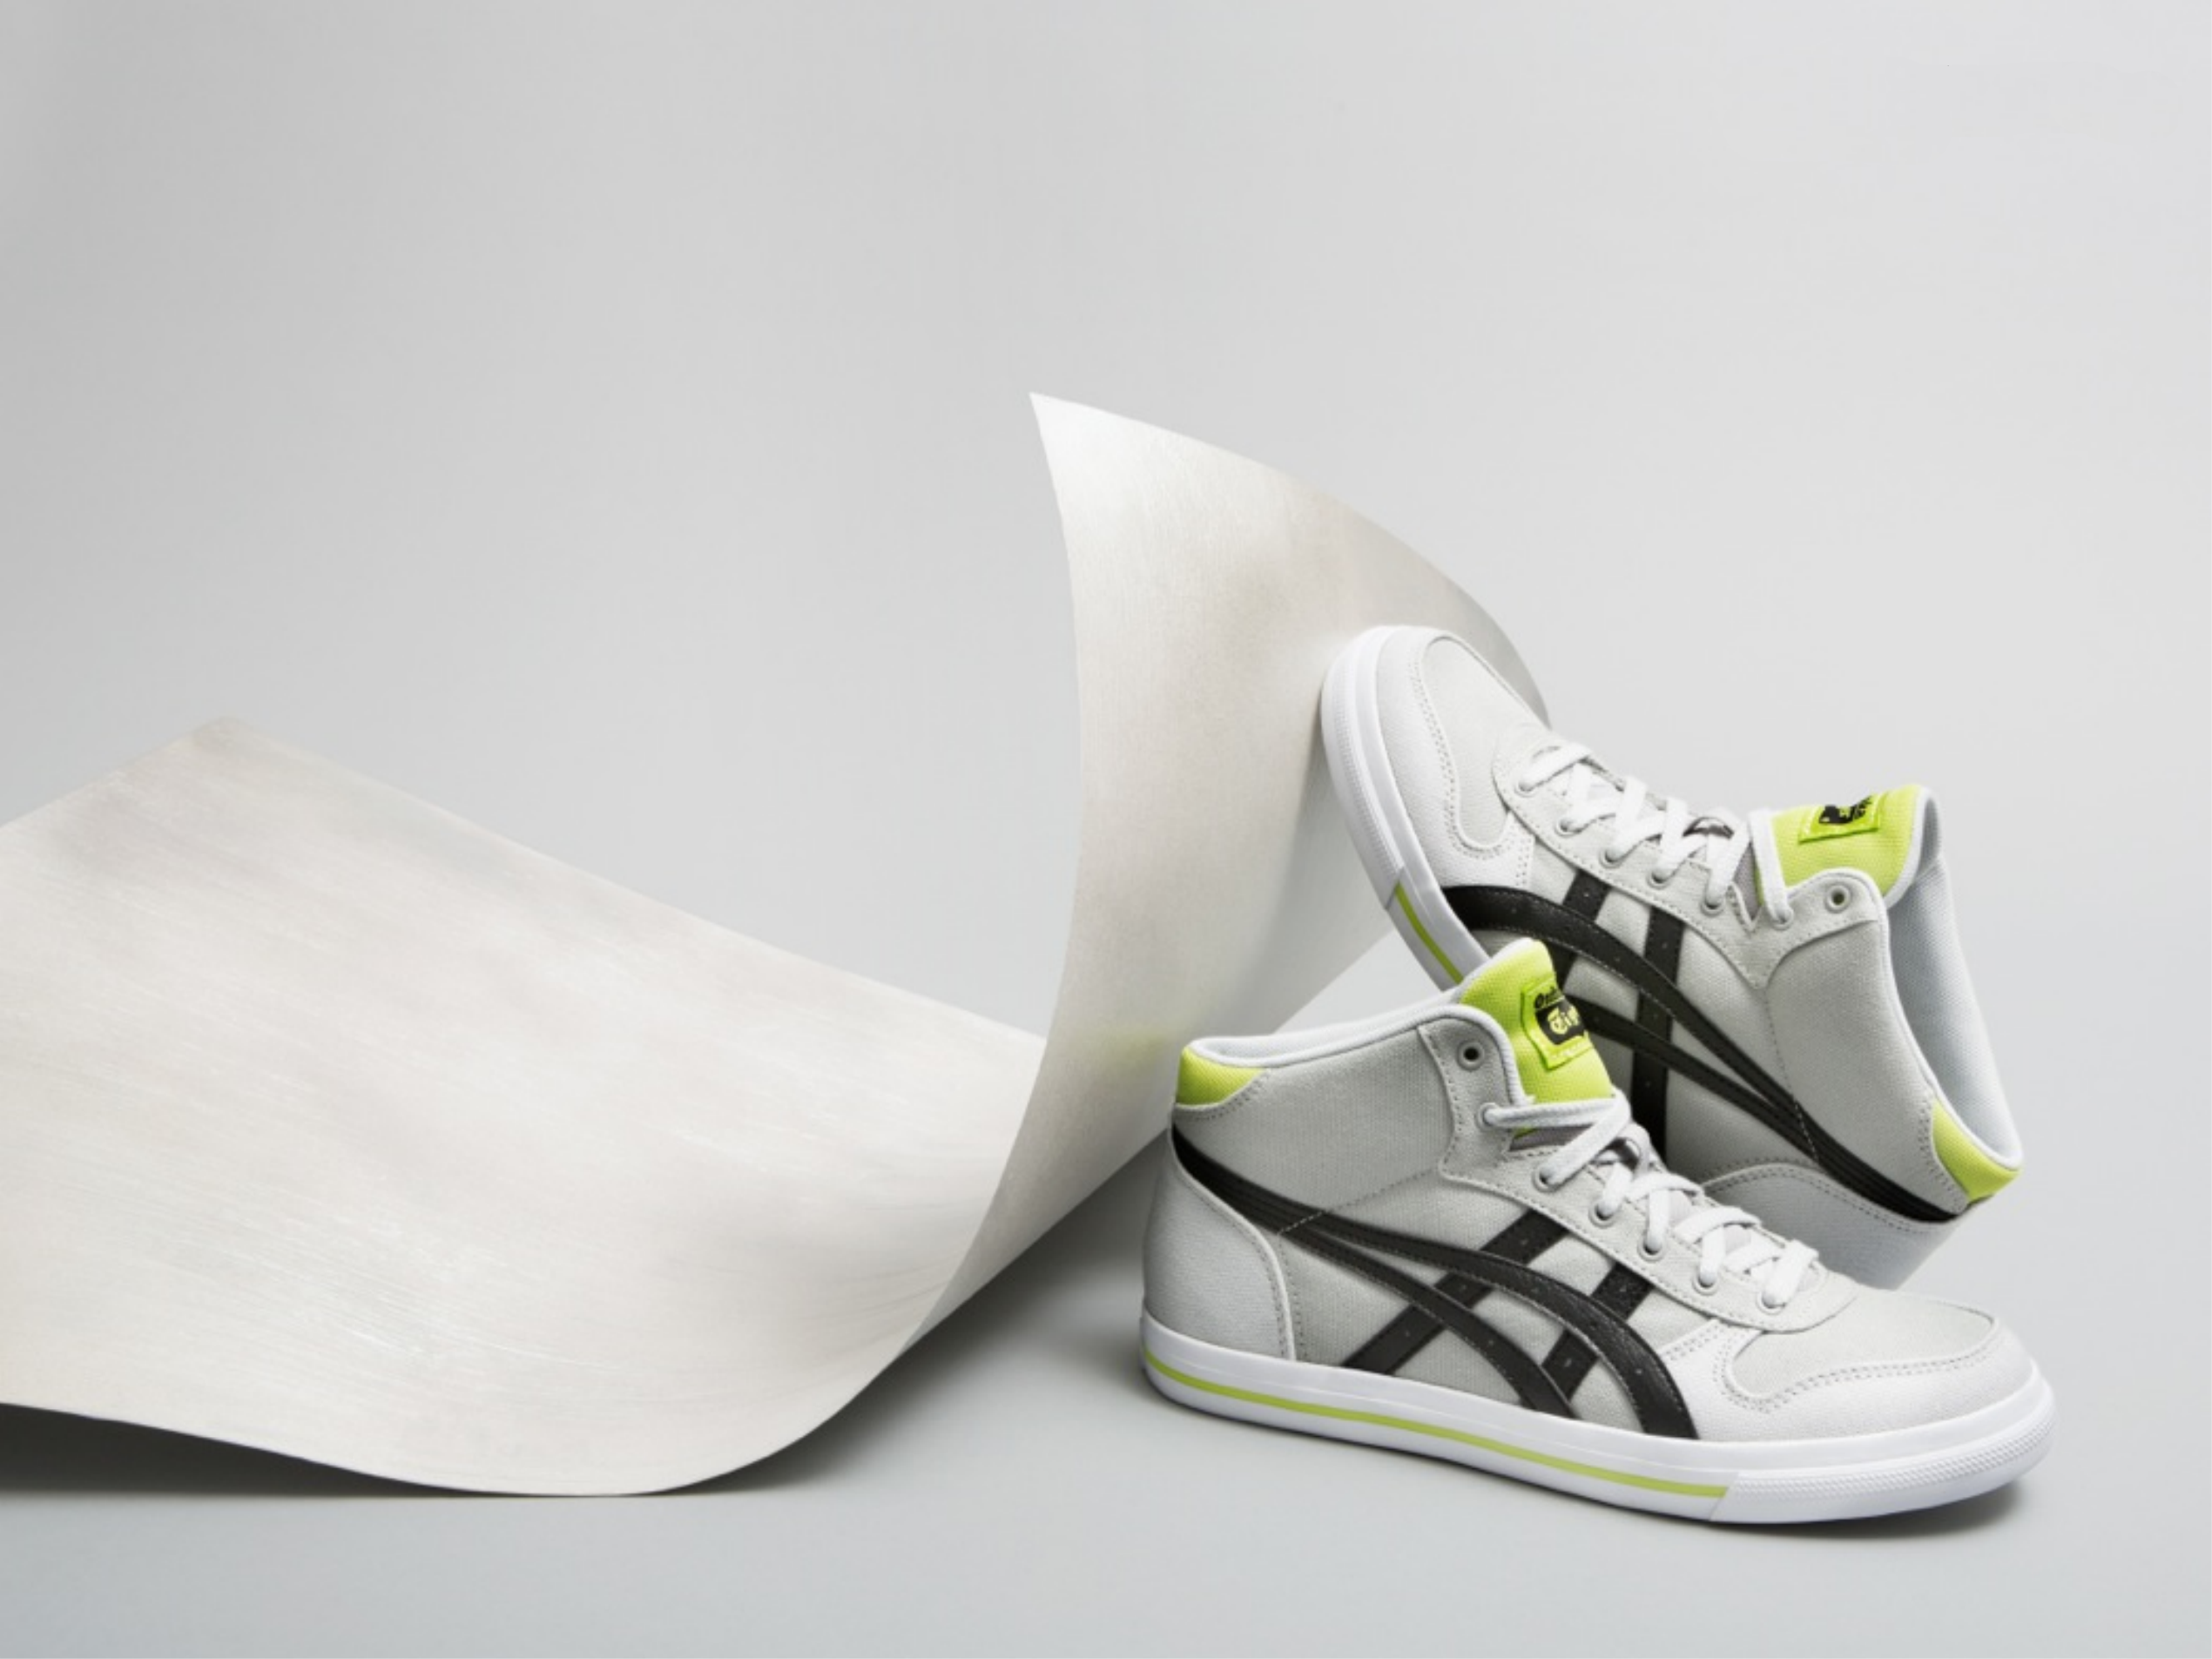
\includegraphics[width=1.1\paperwidth,height=\paperheight]{../figures/reebok_shoes.png}
}
\begin{frame}
  \begin{center}
    \Huge\textbf{Thanks for listening}\\[1cm]
    \Huge\textbf{Get The Slides On\\}
    \LARGE\texttt{github.com/cseward/ocapi\_neural\_net\_blog\_post}
  \end{center}
  \vspace{5cm}
\end{frame}

\end{document}